% =============================================================================
% cs-karnaugh-map.tex — 4-variable Karnaugh map with a grouped implicant
%
% Shows: a 4x4 K-map over AB (rows) and CD (columns) in Gray-code order, with
% one 4-cell group circled and its reduced product term named.
% Compiles standalone via: xelatex cs-karnaugh-map.tex
%
% Use for: digital logic (SOP/POS minimisation), computer organization
% (control-signal simplification), Boolean algebra.
%
% GRAY-CODE ORDER IS THE WHOLE POINT: rows and columns must run 00, 01, 11, 10
% so that adjacent cells differ in exactly one variable. Do not "fix" this to
% binary counting order — it breaks the adjacency the method depends on.
% =============================================================================

\documentclass[border=6pt]{standalone}
\usepackage{tikz}
\usetikzlibrary{arrows.meta, positioning, fit}

\definecolor{grid-line}{HTML}{525252}
\definecolor{header}{HTML}{012169}
\definecolor{group}{HTML}{B91C1C}
\definecolor{cell-fill}{HTML}{E8EDF5}

\tikzset{
  kcell/.style={
    draw=grid-line, fill=white,
    minimum width=1.1cm, minimum height=1.1cm, align=center, font=\small
  },
  khead/.style={font=\small\bfseries, text=header},
  kgroup/.style={draw=group, very thick, rounded corners=6pt}
}

% -----------------------------------------------------------------------------
% Diagram: 4-variable K-map, F(A,B,C,D). Cell (col i, row j) sits at
%   x = 1.1*i, y = -1.1*j   for i, j in 0..3
% Column order (CD): 00, 01, 11, 10   <- Gray code
% Row order    (AB): 00, 01, 11, 10   <- Gray code
% Axis headers sit 0.85cm outside the grid so they never touch a cell border
% (P7c). The circled group covers the two RIGHT columns of the two BOTTOM rows
% -- cells (11,11) (11,10) (10,11) (10,10) -- i.e. A=1 and C=1, reducing to AC.
% The group rectangle is drawn with `fit` over those four cell nodes plus 3pt
% padding, so it hugs the cells without overlapping neighbouring text.
% -----------------------------------------------------------------------------

\begin{document}
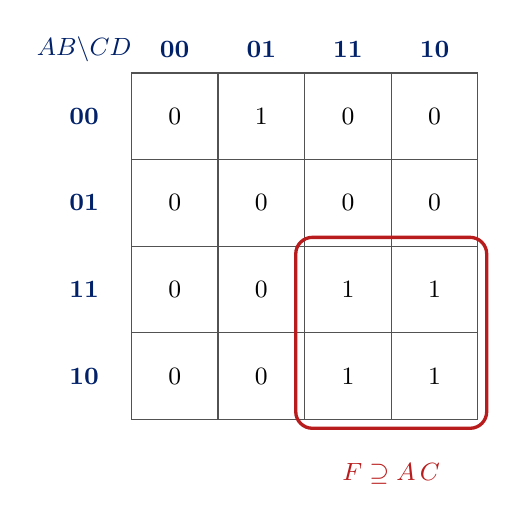
\begin{tikzpicture}

  % ---- Cells: values of F -------------------------------------------------
  % Row/col labels in Gray-code order
  \def\colvals{{"00","01","11","10"}}
  \def\rowvals{{"00","01","11","10"}}

  % F values, row-major, rows AB = 00,01,11,10 and cols CD = 00,01,11,10
  % F = 1 wherever A=1 AND C=1 (the group), plus one isolated minterm at
  % AB=00, CD=01 to show a non-grouped 1.
  \def\vals{{
    {0,1,0,0},
    {0,0,0,0},
    {0,0,1,1},
    {0,0,1,1}}}

  \foreach \j in {0,1,2,3} {
    \foreach \i in {0,1,2,3} {
      \pgfmathparse{\vals[\j][\i]}\edef\cellval{\pgfmathresult}
      \node[kcell] (c\i-\j) at (1.1*\i, -1.1*\j) {\cellval};
    }
  }

  % ---- Column headers (CD), above the grid --------------------------------
  \foreach \i in {0,1,2,3} {
    \pgfmathparse{\colvals[\i]}\edef\lbl{\pgfmathresult}
    \node[khead] at (1.1*\i, 0.85) {\lbl};
  }
  \node[khead] at (-1.15, 0.85) {$AB\backslash CD$};

  % ---- Row headers (AB), left of the grid ---------------------------------
  \foreach \j in {0,1,2,3} {
    \pgfmathparse{\rowvals[\j]}\edef\lbl{\pgfmathresult}
    \node[khead] at (-1.15, -1.1*\j) {\lbl};
  }

  % ---- The implicant group: A=1, C=1  ->  AC ------------------------------
  \node[kgroup, fit=(c2-2)(c3-2)(c2-3)(c3-3), inner sep=3pt] (g) {};
  \node[font=\small\bfseries, text=group, below=0.30cm of g] {$F \supseteq A\,C$};

\end{tikzpicture}
\end{document}
